\section{Process Pipeline}
\label{sec:process_pipeline}

The whole process of fault estimation can be seen as a pipeline. We start at the most basic starting block, the camera streams, and end at the most complex block, the fault estimation. The pipeline is shown in Figure \ref{fig:process_pipeline}. The pipeline consists of seven steps, which are described in more detail in the following sections. The steps are (\textbf{I}) Stream Pre-Processing, (\textbf{II}) Data Acquisition, (\textbf{III}) Data Population, (\textbf{IV}) Data Post-Processing/Evaluation, (\textbf{V}) Data Augmentation, (\textbf{VI}) Model Training, and (\textbf{VII}) Model Evaluation. The results of each step are used as input for the next step. 

We further divided the process into a data processing and model development phase. The data processing phase is the first five steps of the pipeline. The model development phase is the last two steps of the pipeline.

In the next chapters, we give a basic overview of the whole process. We go into more detail in the following sections.

\begin{figure}[ht]
    \centering
    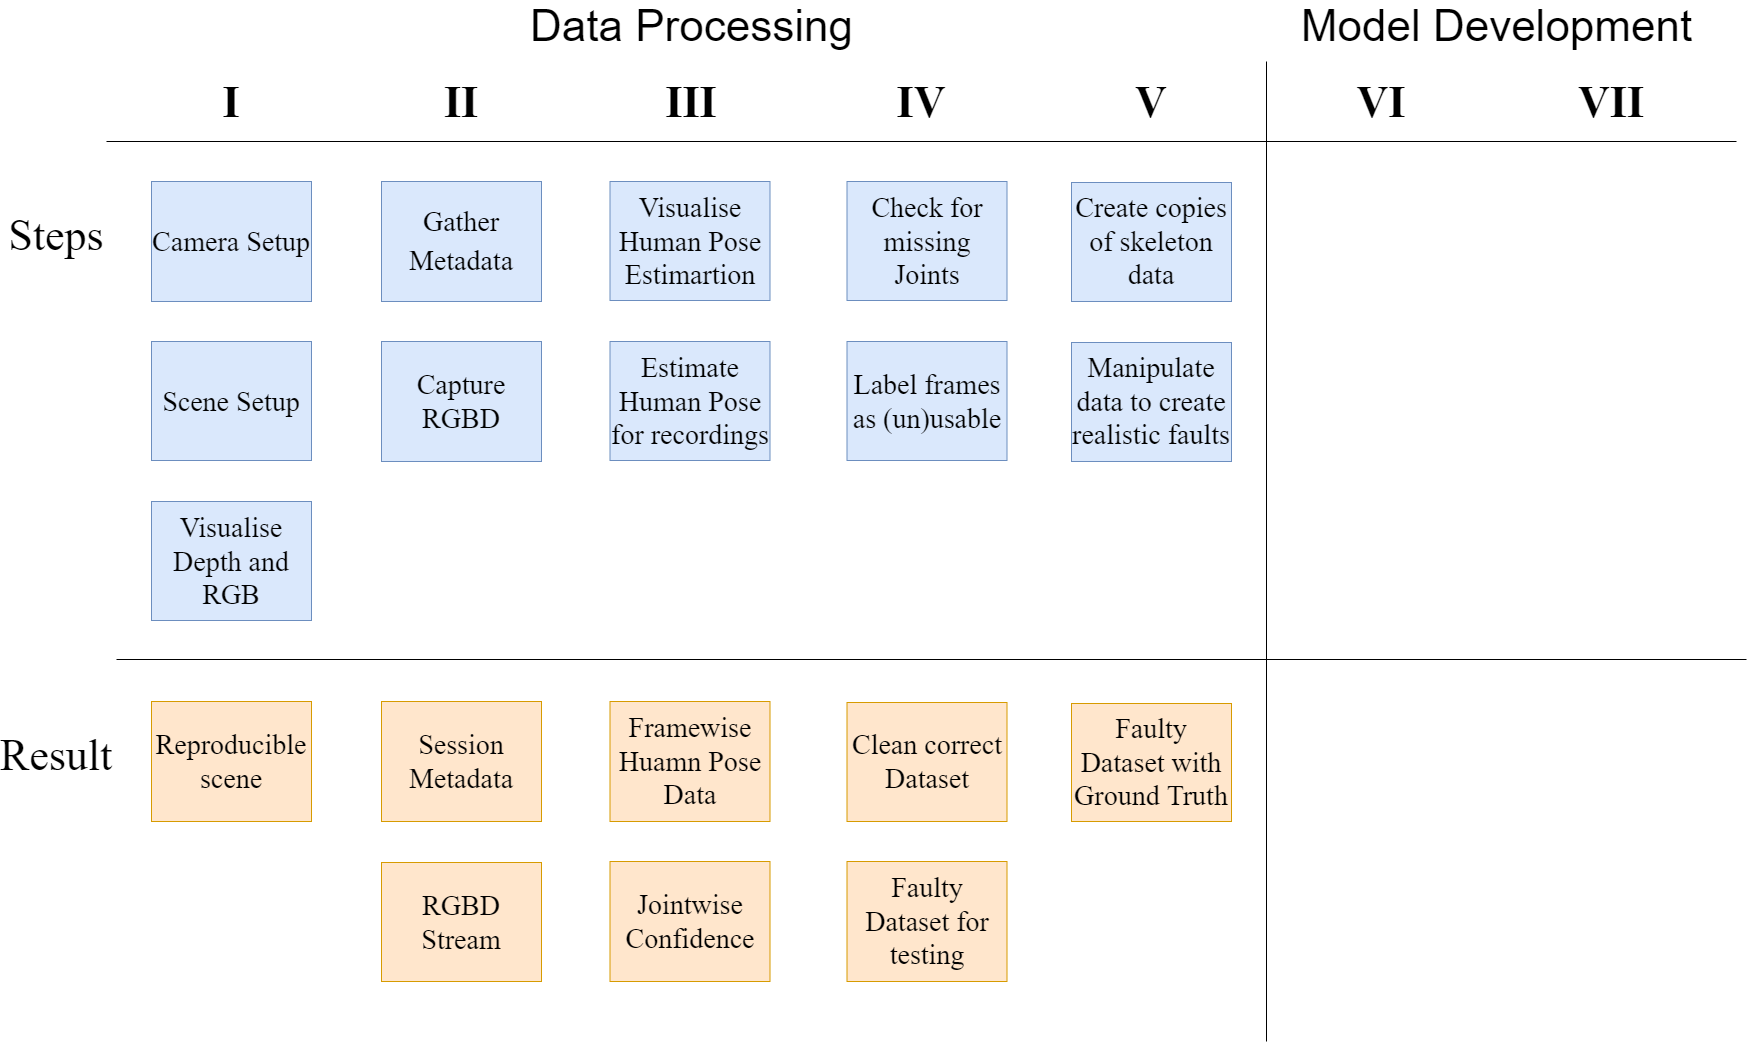
\includegraphics[width=\textwidth]{figures/ProcessingPipeline/ProcessingPipeline.png}
    \caption[Process Pipeline with all steps]{The whole Process pipeline with all the steps, which are marked in blue, and the results of each step, which are marked orange. The results of the steps are used as input for the next step. The steps are described in more detail in the following sections. The steps are: (\textbf{I}) Stream Pre-Processing, (\textbf{II}) Data Acquisition, (\textbf{III}) Data Population, (\textbf{IV}) Data Post-Processing/Evaluation, (\textbf{V}) Data Augmentation, (\textbf{VI}) Model Training, and (\textbf{VII}) Model Evaluation.}
    \label{fig:process_pipeline}
\end{figure}
